%!TEX root = ../TechnischerEntwurf.tex

\chapter{Resultierende Softwarearchitektur}\label{chap:architektur}

Dieser Abschnitt hat die Aufgabe, einen Überblick über die zu entwickelnden
Komponenten und Subsysteme zu liefern.

\section{Komponentenspezifikation}

\begin{figure}[ht]
\centering
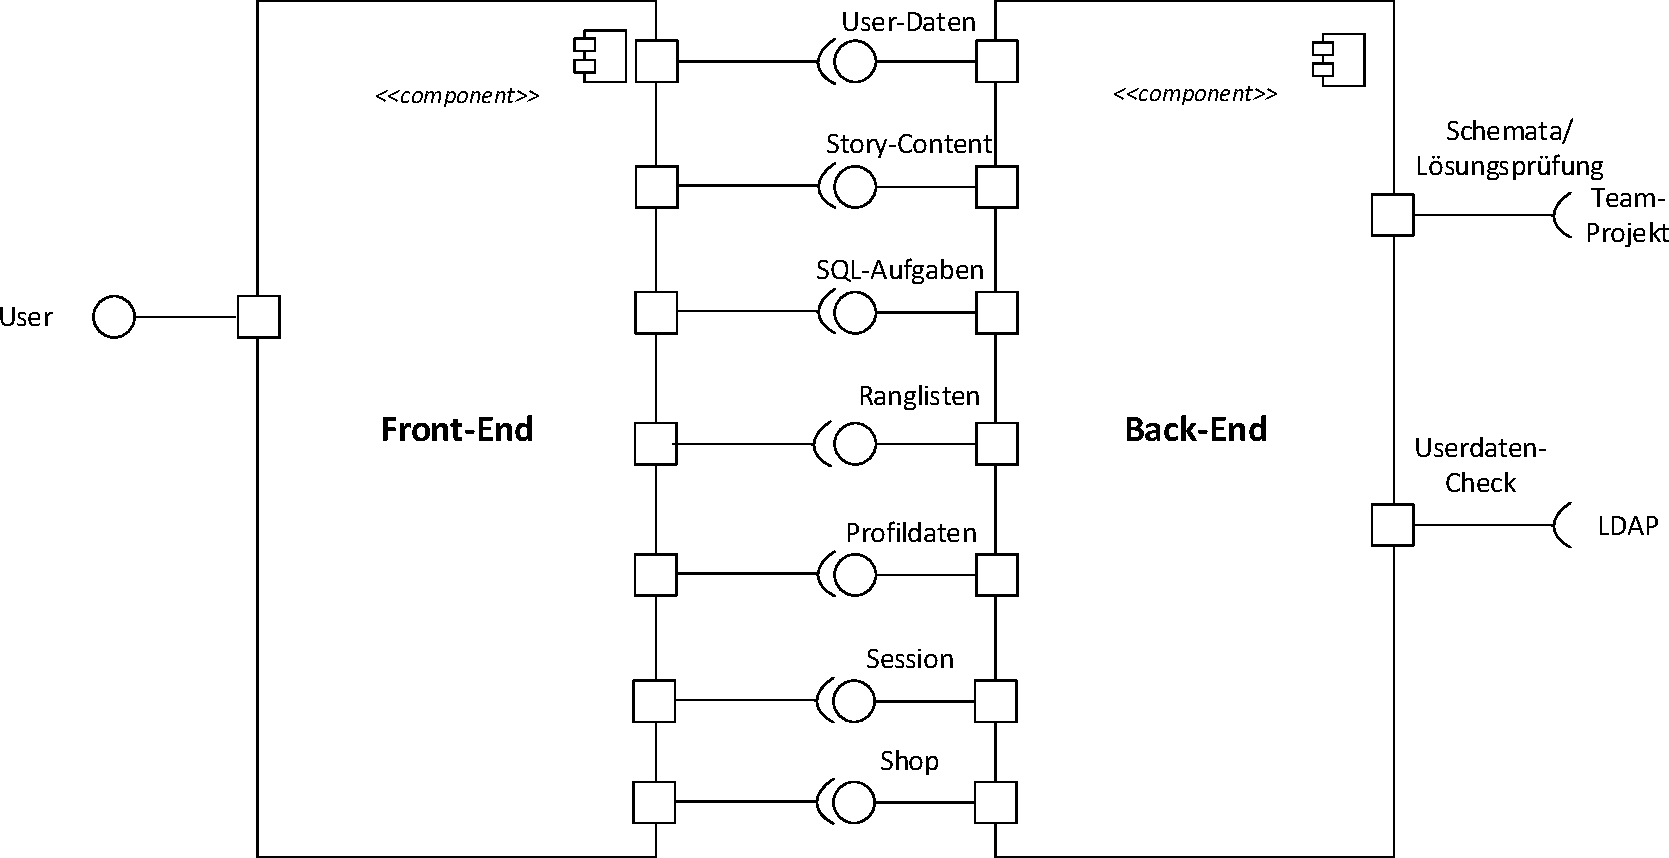
\includegraphics[width=1\textwidth]{figures/komponenten_anfang.pdf}
\caption{Komponentendiagramm.}
\label{component}
\end{figure}

\newpage
In Abbildung 3.1 ist das Komponentendiagramm zu sehen, das sich aus der Funktionionsanalyse in Abschnitt 2 ergibt. Darin ist zu erkennen, dass die beiden Komponenten, Front-End und Back-End, über verschiedene Interfaces miteinander kommunizieren. Des Weiteren ist zu sehen, dass das Back-End eine Anbindung an das LDAP benötigt, um einen Teil der Nutzerdaten überprüfen zu können. 


\begin{component}{10}{<Front-End>}
Das Front-End ist ein Interface, das sämtliche vom Back-End angeforderten Daten verarbeitet. Dazu gehört die entsprechende Visualisierung dieser Daten. Das Front-End ist also die Oberfläche der Software, die der User sieht.
\end{component}

\begin{component}{20}{<Back-End>}
Das Back-End ist eine Datenbank, die dem Front-End verschiedene Schnittstellen zur Verfügung stellt, um an die angeforderten Daten zu kommen.
\end{component}

\newpage
\section{Schnittstellenspezifikation}

Im Folgenden werden die einzelnen Schnittstellen der Komponenten aus der
Komponentenspezifikation näher erläutert, d.h. die von ihnen zur Verfügung
gestellten Operationen werden dokumentiert. Die Tabelle ist dabei um so viele
Zeilen zu erweitern, wie es Schnittstellen im Komponentendiagramm gibt. In der
innen liegenden Aufteilung ist für jede Operation einer Schnittstelle eine
Zeile einzufügen.  Reine Set- und Get-Aufrufe brauchen nicht aufgeführt zu
werden (sollten auch möglichst nicht komponentenübergreifend auftauchen).

\begin{interface}{10}{<Session>}

\begin{center}
	\begin{tabular}[h]{|c|c|c|c|c|}
	\hline
	\textbf{Action and URL} &\textbf {Method} &\textbf {Send} &\textbf {Response Success} & \textbf{Response Error}\\
	\hline
	POST    /login & .create  & JSON.login  & redirect(/profile)  & 401(JSON.sign.error) \\
	\hline
	GET     /logout & .delete & - & ok & - \\
	\hline
	 \end{tabular}
\end{center}

\end{interface}

Möchte sich ein User einloggen, sendet das Front-End ein JSON-Objekt mit den Login-Daten an das Back-End. Es wird versucht mittels der \glqq create \grqq -Methode eine Session zu erstellen. Bei Erfolg wird die Session angelegt und der User in den Home-Screen weitergeleitet, wobei die Profildaten bereits geladen werden. Bei Misserfolg wird ein HTTP-Error (hier für unautorisierter User) inklusive eines JSON-Objektes zurückgegeben, welches die Ursache des Fehlers beinhaltet.
Möchte der User sich wieder ausloggen, wird dies per HTTP-GET-Anfrage übermittelt. Daraufhin wird die aktuelle Session durch die \glqq delete\grqq -Methode gelöscht.

\newpage
\begin{interface}{20}{<Userdaten>}

\begin{center}
	\begin{tabular}[h]{|c|c|c|c|c|}
	\hline
	\textbf{Action and URL} &\textbf {Method} &\textbf {Send} &\textbf {Response Success} & \textbf{Response Error}\\
	\hline
	POST     /signup & .create & JSON.signup & redirect(/login) & 400(JSON.sign.error)\\
	\hline
	POST     /users & .edit & JSON.user & ok & 400(JSON.sign.error)\\
	\hline
	DELETE     /users & .delete & - & ok & 400(JSON.sign.error)\\
	\hline
	 \end{tabular}
\end{center}

\end{interface}

Möchte sich ein User registrieren, wird ein JSON-Objekt mit den entsprechenden Daten an das Back-End gesendet, welches daraufhin mittels der \glqq create \grqq -Methode versucht einen neuen User zu erstellen. Bei Erfolg wird der User angelegt und dieser kann sich im Login-Screen einloggen. Bei Misserfolg wird ein HTTP-Error (Bad request) inklusive eines JSON-Objektes zurückgegeben, welches die Ursache für die Fehlermeldung beinhaltet.
Außerdem kann der User sein Passwort ändern. Das vom User eingegebene alte und neue Passwort wird per JSON-Objekt an das Back-End ünbermittelt. Dort wird das alte Passwort überprüft. Ist es korrekt, wird das neue Passwort gespeichert, ist es nicht korrekt, wird ein HTTP-Error (Bad request) inklusive eines JSON-Objektes zurückgegeben, welches die Ursache des Fehlers beinhaltet.
Möchte der User seinen Account löschen, muss er sein Passwort eingeben. Dieses wird dann per JSON-Objekt an das Back-End gesendet. Bei korrektem Passwort wird der User gelöscht, bei inkorrektem Passwort wird ein Fehler (Bad request) inklusive eines JSON-Objektes zurückgegeben, welches die Ursache des Fehlers beinhaltet.

\newpage
\begin{interface}{40}{<SQL-Aufgaben>}
Challenge
\begin{center}
	\begin{tabular}[h]{|c|c|c|c|c|}
	\hline
	\textbf{Action and URL} &\textbf {Method} &\textbf {Send} &\textbf {Response Success} & \textbf{Response Error}\\
	\hline
	GET     /challenge & .index & - & JSON.challenge[ ] & - \\
	\hline
	GET     /challenge/:id & .view  & - & JSON.challenge & - \\
	\hline
	POST     /challenge & .create & JSON.challenge & ok & - \\
	\hline
	GET     /challenge/story & .story & - & JSON.story  & - \\
	\hline
	GET     /challenge/trivia & .trivia  & - & JSON.task & - \\
	\hline
	GET     /challenge/homework & .homework & - & JSON.task & - \\
	\hline
	 \end{tabular}
\end{center}

Im Admin-Tool können die Administratoren die vorhandenen Challenges betrachten oder neue erstellen.
Dabei kann der Admin entweder alle Challenges, eine Challenge mit einer bestimmten ID oder alle Challenges eines bestimmten Typs anzeigen lassen.
Eine neue Challenge wird im JSON Format an das Back-End gesendet und dort gespeichert.

\newpage
Task
\begin{center}
	\smaller
	\begin{tabular}[h]{|c|c|c|c|c|}
	\hline
	\textbf{Action and URL} &\textbf {Method} &\textbf {Send} &\textbf {Response Success} & \textbf{Response Error}\\
	\hline
	GET     /tastk/story/:id & .story & -  & JSON.task  & - \\
	\hline
	POST     /task/story/:id & .storySolve & JSON.task.solve & JSON.task.result & 400(JSON.task.result) \\
	\hline
	GET     /task/trivia & .triva & - & JSON.task & - \\
	\hline
	POST     /task/trivia/:id & .triviaSolve & JSON.task.solve  & JSON.task.result & 400(JSON.task.result) \\
	\hline
	GET     /task/homework & .homework & - & JSON.task & - \\
	\hline
	POST     /task/homework/:id & .homeworkSolve & JSON.task.solve & JSON.task.result & 400(JSON.task.result) \\
	\hline
	GET     /task/ & .index & - & JSON.task[ ] & - \\
	\hline
	GET     /task/:id & .view & - & JSON.task & - \\
	\hline
	POST     /task/:id & .edit & JSON.task & ok & - \\
	\hline
	POST     /task/:id/rating & .rate & JSON.rating & ok & - \\
	\hline
	GET     /task/:id/comment & .comments & - & JSON.comment[ ] & - \\
	\hline
	POST     /task/:id/comment & .comment  & JSON.comment  & - & - \\
	\hline
	 \end{tabular}
\end{center}

\end{interface}

Es gibt mehrere Aufgabentypen, welche übermittelt werden müssen. Story sind Aufgaben für Scrolls mit einer gewissen ID. Die Aufrufe Trivia und Homework starten die Bearbeitung eines Aufgabenpaketes. Die /'solve/' Anfragen sind Antworten des Users auf die Statements mit einer bestimmten ID, die im JSON-Format übergeben werden. Bei richtiger Antwort wird ein JSON-Objekt übergeben, welches diese Information enthält. Bei falscher Antwort wird ein HTTP-Error inklusive eines JSON-Objektes zurückgegeben, welches die Ursache des Fehlers beinhaltet (hier die falsche Antwort). 

\newpage
\begin{interface}{50}{<Ranglisten>}

\begin{center}
	\begin{tabular}[h]{|c|c|c|c|c|}
	\hline
	\textbf{Action and URL} &\textbf {Method} &\textbf {Send} &\textbf {Response Success} & \textbf{Response Error}\\
	\hline
	GET     /highscore/points & .byPoints & - & JSON.highscore[ ]  & - \\
	\hline
	\hline
	GET     /highscore/time & .byTime & - & <JSON.highscore[ ] & - \\
	\hline
	\hline
	GET     /highscore/runs & .byRuns & -  & <JSON.highscore[ ] & - \\
	\hline
	\hline
	GET     /highscore/sql & .bySQL & - & <JSON.highscore[ ] & - \\
	\hline
	\hline
	GET     /highscore/rate & .byRate & - & <JSON.highscore[ ] & - \\
	\hline
	 \end{tabular}
\end{center}

\end{interface}

Hiermit können die Ranglisten in bestimmter Sortierung zurückgegeben werden. Die Rückgabe erfolgt im JSON-Format.

\begin{interface}{60}{<Profildaten>}

\begin{center}
	\begin{tabular}[h]{|c|c|c|c|c|}
	\hline
	\textbf{Action and URL} &\textbf {Method} &\textbf {Send} &\textbf {Response Success} & \textbf{Response Error}\\
	\hline
	GET     /profile & .index & - & JSON.playerstate & - \\
	\hline
	\hline
	GET     /profile/:id & .view & - & JSON.profile & - \\
	\hline
	\hline
	GET     /profile/character & .character & - & JSON.characterState  & - \\
	\hline
	\hline
	GET     /profile/inventory & .inventory & - & JSON.inventory & - \\
	\hline
	 \end{tabular}
\end{center}

\end{interface}

Die Profildaten werden zu Beginn der Session, direkt nach dem login, vom Back-End angefordert. Das JSON-Objekt enthält den Benutzernamen, aktuelle Einstellungen, ob der User ein Student ist oder nicht, die aktuellen coins und wie nahe der User an den täglichen Limits für coins/scrolls ist.
Es können auch die Profile anderer Benutzer betrachtet werden, dies erfolgt über die Profil-ID.
Der /'characterState/' ist für das Minispiel von Relevanz, es wird ein JSON-Objekt übergeben, welches die Attribute, gekaufte Avatare und den aktuellen Avatar enthält.


\begin{interface}{60}{<Shop>}

\begin{center}
	\begin{tabular}[h]{|c|c|c|c|c|}
	\hline
	\textbf{Action and URL} &\textbf {Method} &\textbf {Send} &\textbf {Response Success} & \textbf{Response Error}\\
	\hline
	GET     /shop & .index  & -  & JSON.shopitem[ ] & - \\
	\hline
	\hline
	POST    /shop/:id & .buy & -  & ok & 400 \\
	\hline
	 \end{tabular}
\end{center}

\end{interface}

Wenn der Benutzer auf den Shop klickt, holt sich das Front-End die gesamte Liste der Shopitems in Form eines JSON-Arrays, um sie für den Benutzer darzustellen. 


\newpage
\section{Protokolle für die Benutzung der Komponenten}

Abbildung \ref {state_game} stellt ein Statechart für die Front-End-Komponente (C10) dar. Darauf folgt eine Beschreibung zur Verwendung der Komponente, sodass beides hier nicht mehr erfolgen muss. 

\begin{figure}[ht]
\centering
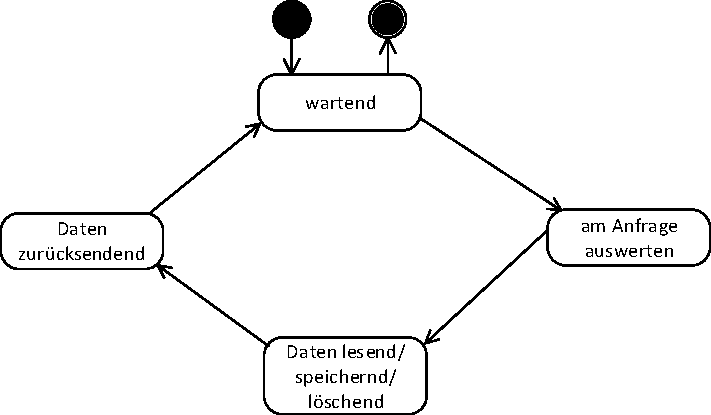
\includegraphics[width=1\textwidth]{figures/statechart_BE.pdf}
\caption{Back End - Statechart}
\label{be-state}
\end{figure}

In Abbildung \ref {be-state} sind die Zustände des Back-Ends (C20) dargestellt.
Das Back-End ist eine Datenbank, die auf Anfragen wartet. Erfolgt eine Anfrage an das Back-End, wird diese zuerst ausgewertet, um herauszufinden was getan werden soll. Ist dies geschehen, wird die geforderte Aktion umgesetzt und je nach Art der Aktion und Erfolg oder Misserfolg wird entweder der angeforderte Datensatz oder eine Mitteilung zurückgesendet. 

Grundlegend sollte es möglich sein, sowohl das Front-End (C10), als auch das Back-End (C20) wiederzuverwenden. Dabei ist anzumerken, dass die im Front-End angezeigten Daten alle im Back-End lagern, wodurch eine gemeinsame Wiederverwendung am sinnvollsten erscheint. Das Austauschen des SQL-Trainers gegen einen anderen zu erlernenden Inhalt sollte auch möglich sein, wenn sich die Aufgaben in das hier verwendete Schwierigkeitsgrad-Schema (5 Schwierigkeitsgrade) einpassen lassen. 

%In diesem Abschnitt wird mit Hilfe von Protokoll-Statecharts die korrekte
%Verwendung der zu entwickelnden Komponenten dokumentiert. Dies ist insbesondere
%für diejenigen Komponenten notwendig, für die eine Wiederverwendung möglich
%erscheint oder sogar bereits geplant ist.
%
%Begründen Sie für welche Komponenten eine Wiederverwendung sinnvoll erscheint
%und für welche nicht!
%Fügen Sie so viele Statechartdiagramme ein, wie sie Komponenten gefunden haben.
